\documentclass{article}
\usepackage[T1]{fontenc}
\usepackage{tgbonum}
\usepackage{float}
\renewcommand{\familydefault}{\sfdefault}
\usepackage[T1]{fontenc}
\usepackage{varioref}
\usepackage[utf8]{inputenc}
\usepackage{tabularx,ragged2e,booktabs,caption}
\newcolumntype{C}[1]{>{\Centering}m{#1}}
    
% Language setting
% Replace `english' with e.g. `spanish' to change the document language
\usepackage[english]{babel}

% Set page size and margins
% Replace `letterpaper' with `a4paper' for UK/EU standard size
\usepackage[letterpaper,top=2cm,bottom=2cm,left=2cm,right=2cm,marginparwidth=1.75cm]{geometry}
\usepackage{amsmath}
\usepackage{graphicx}
\usepackage[colorlinks=true, allcolors=blue]{hyperref}

\title{\textbf{How big is the gender wage gap?}}
\author{Jiaxiang Chen}
\date{}



\begin{document}
\maketitle


\section{Introduction}
The wage and the wage inequality have long been known that are complex functions of various soci-economic variables, and gender is an important part of them. The gap, however, has been changing over years and it's important to know how it changes. With the 1990-2012 CPS data, we can take a glimpse into the US gender wage gap over time, especially examine the difference respect to different percentile of the wage and education.


\section{Data(Q1)}
After dropping the data with missing value, there is 3690 observations and 5 variables : Gender, Race, Age, Education, Year and Hourly wage (unadjusted for inflation). With the given deflation data, we can obtain the real wage using 2012 price as the base.
\\~\\
The summary statistics after deflating the data is displayed in \textit{Table 1},\\

\begin{minipage}{\linewidth}
\centering
\captionsetup{labelfont=bf}
\captionof{table}{\textbf{Summary Statistics: 1990-2012 CPS}}\label{tab:title}
\begin{tabularx}{\textwidth}{ C{1.25in} C{.85in} *5{C{.75in}}}\toprule[1.5pt]
 \textbf{Numerical Variable} & \textbf{n} & \textbf{Mean} & \textbf{Median} & \textbf{Max} & \textbf{Min} & \textbf{NA}  \\ 
  \hline 
\hline
  Age & 3690 &   39.6 &   39.0 &   64.0 &   16.0& 0 \\ 
  Hourly\ wage & 3690 &   15.8 &   12.7 &   89.7 &    1.0& 0 \\ 
  Real\ Hourly\ wage & 3690 &   19.2 &   15.7 &   92.5 &    1.3& 0 \\ 
  \hline
\end{tabularx}\par
\end{minipage}
\bigskip

\begin{minipage}{\linewidth}
\centering
\begin{tabularx}{\textwidth}{@{} C{1.25in} C{1.3in} *4X @{}}\toprule[0.5pt]
\textbf{Categorical Variable} & \textbf{Levels} & \textbf{n} & \textbf{Percentage} & $\mathbf{\sum \%}$ \\ 
  \hline
  \hline
Gender & Male & 1881 & 51.0 & 51.0 \\ 
   & Female & 1809 & 49.0 & 100.0 \\ 
   \hline
Race & Black & 333 & 9.0 & 9.0 \\ 
   & Other & 213 & 5.8 & 14.8 \\ 
   & White & 3144 & 85.2 & 100.0 \\ 
   \hline
Education & HS dropout & 401 & 10.9 & 10.9 \\ 
   & HS grad & 1186 & 32.1 & 43.0 \\ 
   & Some Uni& 1048 & 28.4 & 71.4 \\ 
   & Bachelor or higher & 1055 & 28.6 & 100.0 \\ 
   \bottomrule[1.5pt]
\end {tabularx}\par
\end{minipage}
\\~\\
\section{Descriptive Analysis of Gender Wage Gap}
First, we need to explore the characteristics of the variable. Specifically , we first take data of 2012 out to examine it statically and then the whole dataset from a  dynamic perspective.\\

\subsection{2012 Wage Data}
First we examine the 2002 data set statically with respect to different quantiles and education.
\subsubsection{2012 Wage at Different Percentile(Q2)}
The three key percentile of the 2012 wage data and their corresponding ratio.\\~\\
(1) $90^{th}$ percentile: \$35.02\  (2) $50^{th}$ percentile: 16.21\  (3) $10^{th}$ percentile of the wage is \$8.24\\
(1) $90^{th}$/$10^{th}$  ratio: 4.25\   (2) $50^{th}$/$10^{th}$  wage ratio: 1.97.\\~\\
It will be helpful to see the trend of gender wage gap at each percentile. Plus, the wage is not showing a proportional relations with the percentile,implying that we might need to use a logarithm form of the wage in the regression analysis.\\


\subsubsection{2012 Education(Q3)}
Education has always been the most important factor impacting the wage. From 2012 data, we can be inferred that 61.5\% percentage of people who have at least some university education. To see the trend of the gender wage gap, we need to control for the education for different gender and different year.\\

\subsection{1990-2012 Wage Data}
Then we examine the whole data set dynamically with respect to different quantiles and education.
\subsubsection{Distribution of Real Wage by Gender(Q4)}
Firstly, from \textit{Table 2} and \textit{Figure 1},  we see that over the whole 23 years, women in general are more likely to work in the low income job, whilst significantly more high income jobs are occupied by men.
\begin{table}[H]
\centering
\captionsetup{labelfont=bf}
\captionof{table}{\textbf{Distribution of Real Wage by Gender}}\label{tab:title}
\begin{tabular}{rlllllll}
  \hline
 & Min & $10^{th}$ & $25^{th}$  & $50^{th}$ & $75^{th}$ & $90^{th}$ & Max \\ 
  \hline
Female &  1.33 &  7.57 &  9.80 & 13.93 & 20.21 & 29.34 & 92.52 \\ 
  Male &  1.44 &  8.58 & 11.81 & 17.71 & 27.53 & 40.12 & 88.84 \\ 
   \hline
\end{tabular}
\end{table}

\begin{figure}[H]
    \centering
    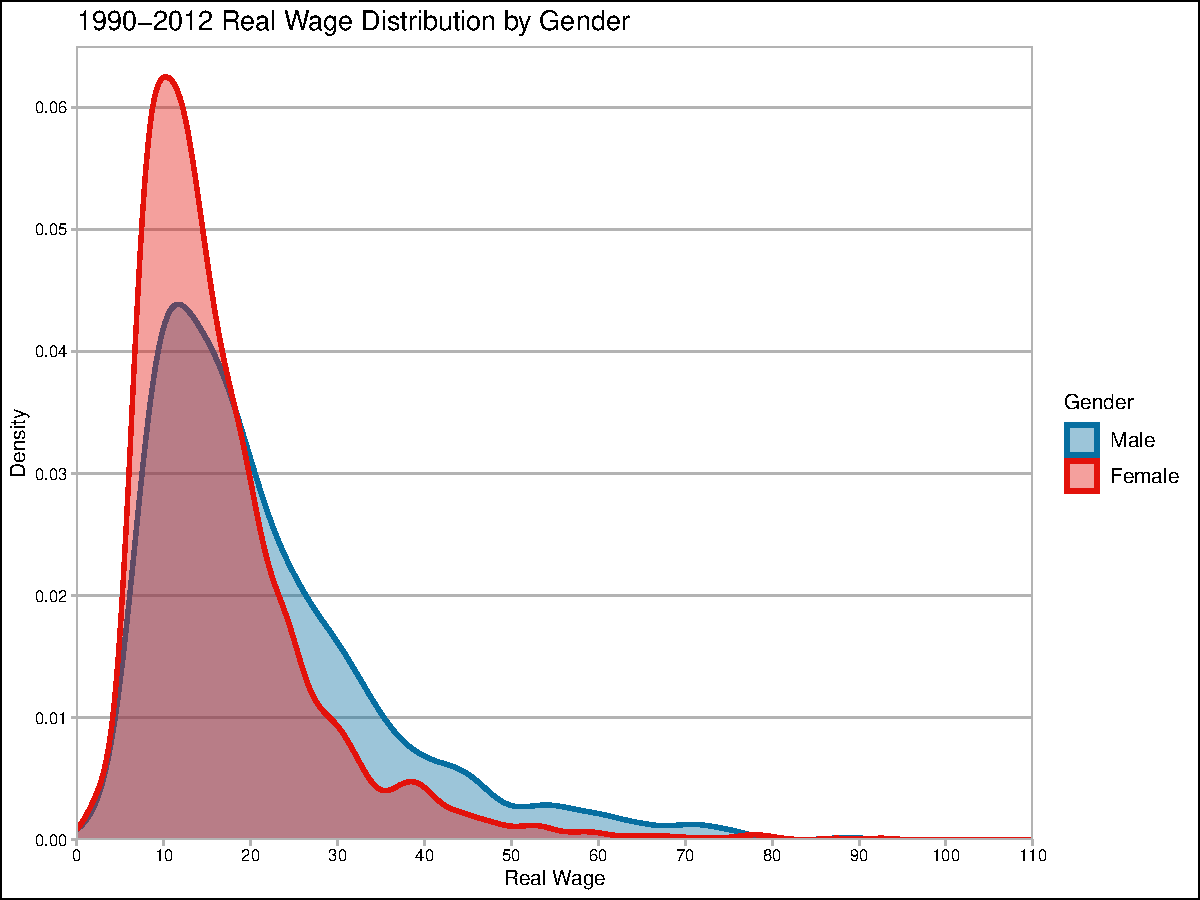
\includegraphics[width=120mm,scale=0.9]{q4p.pdf}
    \caption{1990 - 2012 Real Wage Distribution by Gender}
    \label{fig:my_label}
\end{figure}

\subsubsection{Trend of Wage at Different Percentile(Q5a) }
Then, we look at the trend of wage at different percentile. From \textit{Figure 2}, we can see that for wage of $10^{th}$ and $50^{th}$, they have been very stable around the same level, 8 and 15 dollar per hour respectively. Whilst the wage of $90^{th}$ percentile, there are more fluctuations but generally being stable over the years, around 30 to 40 dollar per hour.
\begin{figure}[H]
    \centering
    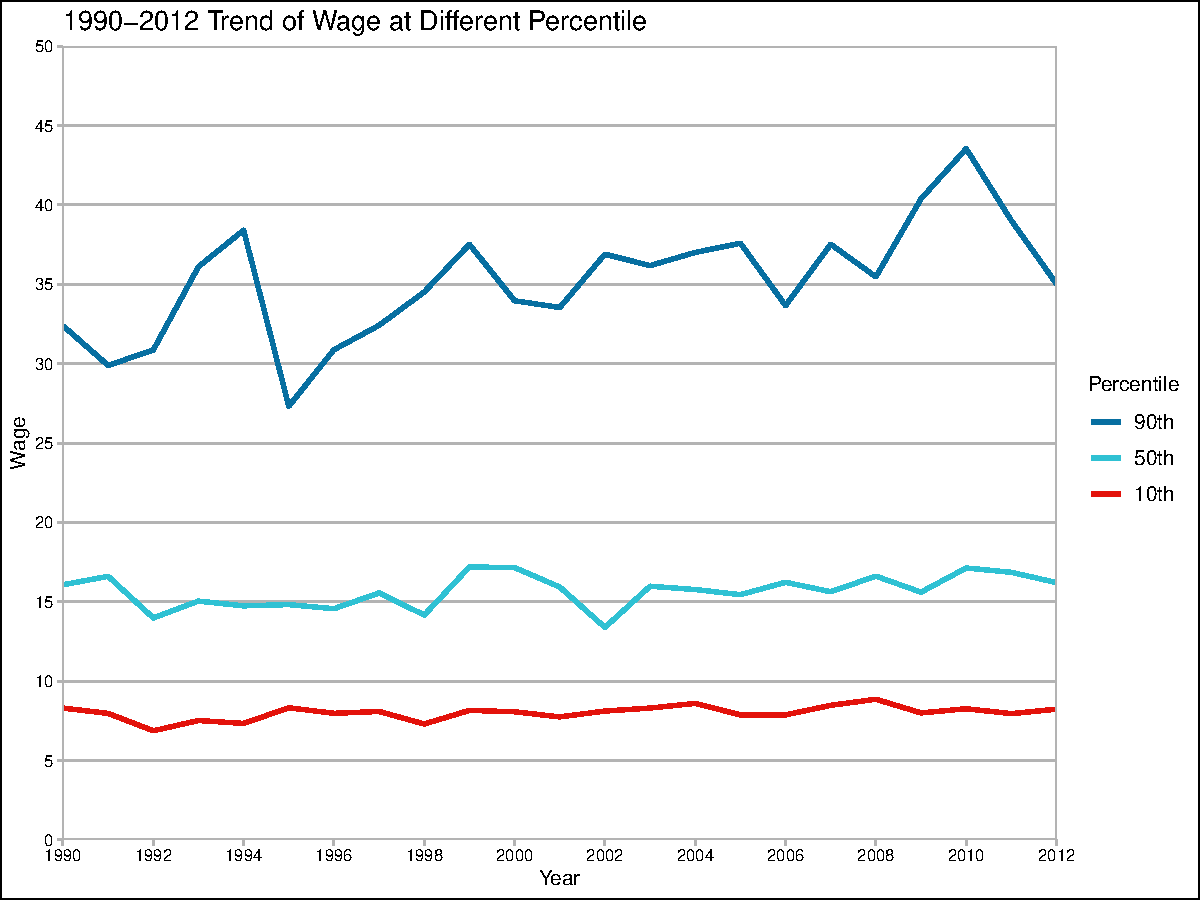
\includegraphics[width=110mm,scale=0.9]{q5p1.pdf}
    \caption{1990 - 2012 Trend of Wage at Different Percentile}
    \label{fig:my_label}
\end{figure}
\subsubsection{Trend of Gender Education Gap(Q5b) }
Finally, we need to look at the gender education difference over the year. From \textit{Figure 3}, we can see that the overall education level of the whole population has been improved. Interestingly, women are gaining the education at a more drastic rate than men, and the sign which women's average education level surpass men's are becoming more obvious recently.\\
\begin{figure}[H]
    \centering
    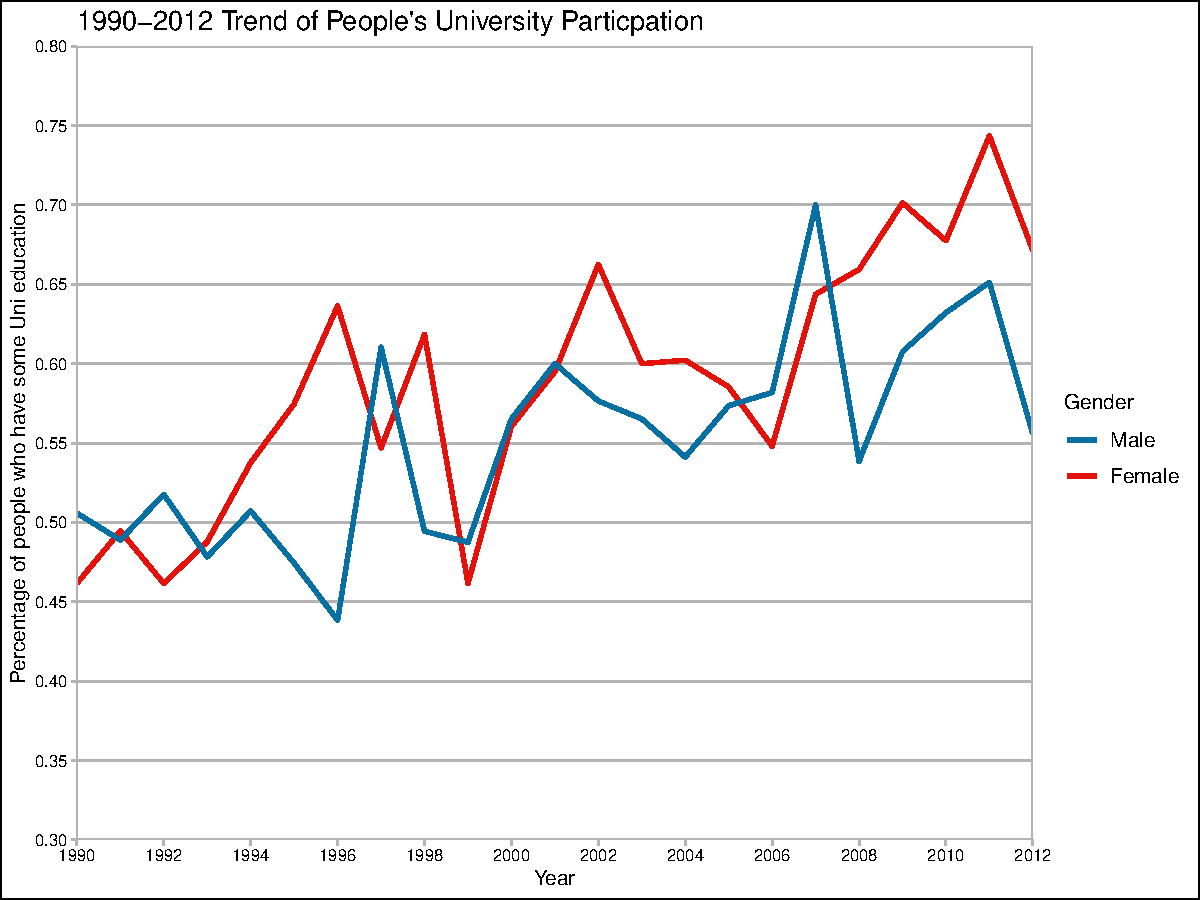
\includegraphics[width=110mm,scale=0.9]{q5p2.pdf}
    \caption{1990 - 2012 Trend of Gender Education Gap}
    \label{fig:my_label}
\end{figure}

\section{Econometric Analysis of Gender Wage Gap}
With above descriptive analysis shows: While the wage at each percentile remaining roughly remaining constant, women are more likely obtain an low income position in general and women are receiving more education. \\~\\
\textit{Question: Is it possible the wage inequality has been declining due to the more education obtainment of women?}.\\

\subsection{Control for Education}
Firstly, we regress the log wage only on gender and then add a dummy to control for education, which is whether the person have some university education or not. Also, there is a third regression which add an additional interaction term of gender and education.\\
\begin{equation}
    LogWage_{i}=\beta_0+\beta_1Gender_i +u_i\newline
\end{equation}
\begin{equation}
    LogWage_{i}=\beta_0+\beta_1Gender+\beta_2SomeUni_i+u_i
\end{equation}
\begin{equation}
    LogWage_{i}=\beta_0+\beta_1Gender+\beta_2SomeUni_i+\beta_3Gender_i*SomeUni_i+u_i
\end{equation}\\
The regression result is shown in the \textit{table 3} below. After controlling education, women earn 24 percent less than men, which is 1 percent more than not controlling the education. Moreover, the interaction term of third regression, though less statistical significant shows that among the people who go to uni, women earn extra 0.01 percent less than men. \\~\
\begin{table}[!htbp] \centering 
\captionsetup{labelfont=bf}
\captionof{table}{\textbf{OLS: Gender Wage Gap and Education}}\label{tab:title}
\begin{tabular}{@{\extracolsep{5pt}}lccc} 
\\[-1.8ex]\hline 
\hline \\[-1.8ex] 
 & \multicolumn{3}{c}{\textit{Dependent variable:}} \\ 
\cline{2-4} 
\\[-1.8ex] & \multicolumn{3}{c}{Log Real Wage} \\ 
\\[-1.8ex] & (1) & (2) & (3)\\ 
\hline \\[-1.8ex] 
 Female & $-$0.234$^{***}$ & $-$0.248$^{***}$ & $-$0.242$^{***}$ \\ 
  & (0.019) & (0.018) & (0.027) \\ 
  & & & \\ 
 Some\ Uni &  & 0.418$^{***}$ & 0.423$^{***}$ \\ 
  &  & (0.018) & (0.025) \\ 
  & & & \\ 
 Female*Some\ Uni &  &  & $-$0.010 \\ 
  &  &  & (0.036) \\ 
  & & & \\ 
 Constant & 2.900$^{***}$ & 2.670$^{***}$ & 2.660$^{***}$ \\ 
  & (0.013) & (0.016) & (0.018) \\ 
  & & & \\ 
\hline \\[-1.8ex] 
Observations & 3,690 & 3,690 & 3,690 \\ 
R$^{2}$ & 0.040 & 0.165 & 0.165 \\ 
Adjusted R$^{2}$ & 0.040 & 0.165 & 0.165 \\ 
Residual Std. Error & 0.573 (df = 3688) & 0.534 (df = 3687) & 0.534 (df = 3686) \\ 
F Statistic & 154.000$^{***}$ (df = 1; 3688) & 365.000$^{***}$ (df = 2; 3687) & 244.000$^{***}$ (df = 3; 3686) \\ 
\hline 
\hline \\[-1.8ex] 
\textit{Note:}  & \multicolumn{3}{r}{$^{*}$p$<$0.1; $^{**}$p$<$0.05; $^{***}$p$<$0.01} \\ 
\end{tabular} 
\end{table}

Additionally, to measure the gender wage gap across percentile and also control for the education, we can run a quantile regression. The result is shown in \textit{Table 4}. The result shows, just like previously mentioned, women in high wage job earn more significantly less than the men, whilst the inequality is moferate for women in lower quantile.
\begin{table}[!htbp] \centering 
\captionsetup{labelfont=bf}
\captionof{table}{\textbf{Quantile Regression: Gender Wage Gap and Education}}\label{tab:title} 
\begin{tabular}{@{\extracolsep{5pt}}lccc} 
\\[-1.8ex]\hline 
\hline \\[-1.8ex] 
 & \multicolumn{3}{c}{\textit{Dependent variable:}} \\ 
\cline{2-4} 
\\[-1.8ex] & \multicolumn{3}{c}{Log Real Wage} \\ 
\\[-1.8ex] & $10^{th}$ & $50^{th}$ & $90^{th}$\\ 
\hline \\[-1.8ex] 
 Female & $-$0.143$^{***}$ & $-$0.250$^{***}$ & $-$0.353$^{***}$ \\ 
  & (0.026) & (0.034) & (0.044) \\ 
  & & & \\ 
 Some\ Uni & 0.254$^{***}$ & 0.445$^{***}$ & 0.510$^{***}$ \\ 
  & (0.035) & (0.038) & (0.044) \\ 
  & & & \\ 
 Female*Some\ Uni & $-$0.008 & $-$0.030 & 0.048 \\ 
  & (0.043) & (0.050) & (0.065) \\ 
  & & & \\ 
 Constant & 2.060$^{***}$ & 2.660$^{***}$ & 3.330$^{***}$ \\ 
  & (0.022) & (0.026) & (0.030) \\ 
  & & & \\ 
\hline \\[-1.8ex] 
Observations & 3,690 & 3,690 & 3,690 \\ 
\hline 
\hline \\[-1.8ex] 
\textit{Note:}  & \multicolumn{3}{r}{$^{*}$p$<$0.1; $^{**}$p$<$0.05; $^{***}$p$<$0.01} \\ 
\end{tabular} 
\end{table}

\subsection{Gender Wage Gap over Time}
\subsubsection{OLS}
To see the gender wage gap change over time, we can use the loop functions in R to obtain the coefficients of all 23 years. Using equation(2), we can run the following equation using the data of each year,
\begin{equation}
    LogWage_{it}=\beta_0+\beta_{1t}Gender+\beta_{2t}SomeUni_{it}+u_{it}
\end{equation}
However, it's difficult to squeeze all the summary statistics in one table, but we can show the trend of key coefficient graphically.
\textit{In Figure 4}, the point indicates the $\beta_{1t}$ of different year. Since higher the point locates indicates less  inequality, we can see gender wage gap decrease from 1990 to 2005,  but increase again later on. It's worth noticing that the trend is not very significant, the coefficient of fitted red line seems to have large standard error.
\begin{figure}[H]
    \centering
    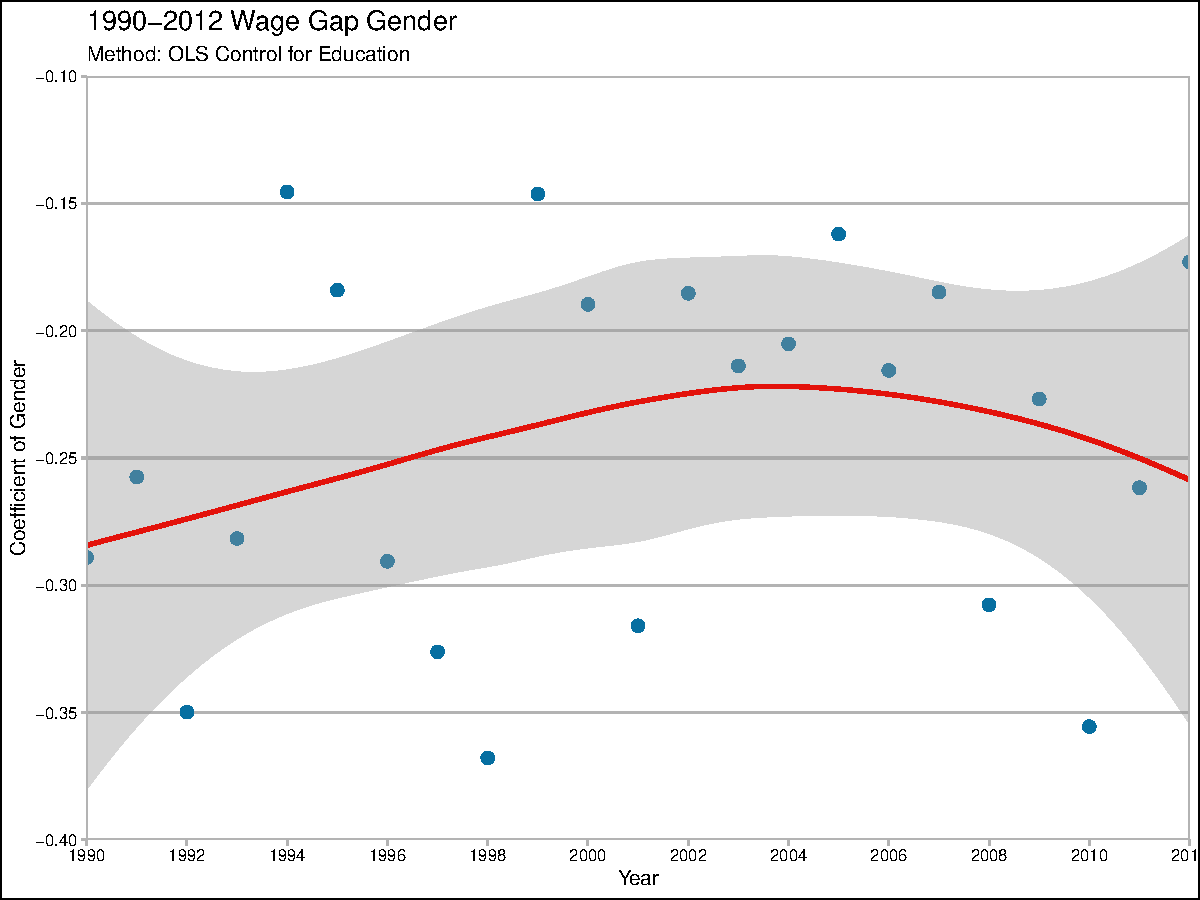
\includegraphics[width=100mm,scale=0.9]{q7p1.pdf}
    \caption{1990 - 2012 Wage Gap Gender(OLS)}
    \label{fig:my_label}
\end{figure}
Also, we can also plot the trend of coefficient for impact of university education. The \textbf{Figure 5 }shoes the trend of it and this time, it shows a similar but more significant result that return to education increase to 2005, but start to decrease then. 
\begin{figure}[H]
    \centering
    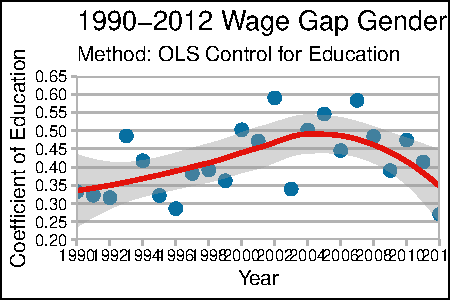
\includegraphics[width=110mm,scale=0.9]{q7p2.pdf}
    \caption{1990 - 2012 Return to Education(OLS)}
    \label{fig:my_label}
\end{figure}
\subsubsection{Quantile Regression}
Also, we can also examine the gender wage gap at different percentile using quantile regression, with controlling  the education. First, we estimate the regression 5 using the each year data and plot the result. In \textit{Figure 6}, it shows that gender wage gap for lowest tier (10th) is decreasing over the years, whilst the inequality between gender has widen for 50th and especially 90th.\\
\begin{equation}
    LogWage_{iqt}=\beta_0+\beta_{1qt}Gender+\beta_{2qt}SomeUni_{iqt}+u_{it}
\end{equation}

\begin{figure}[H]
    \centering
    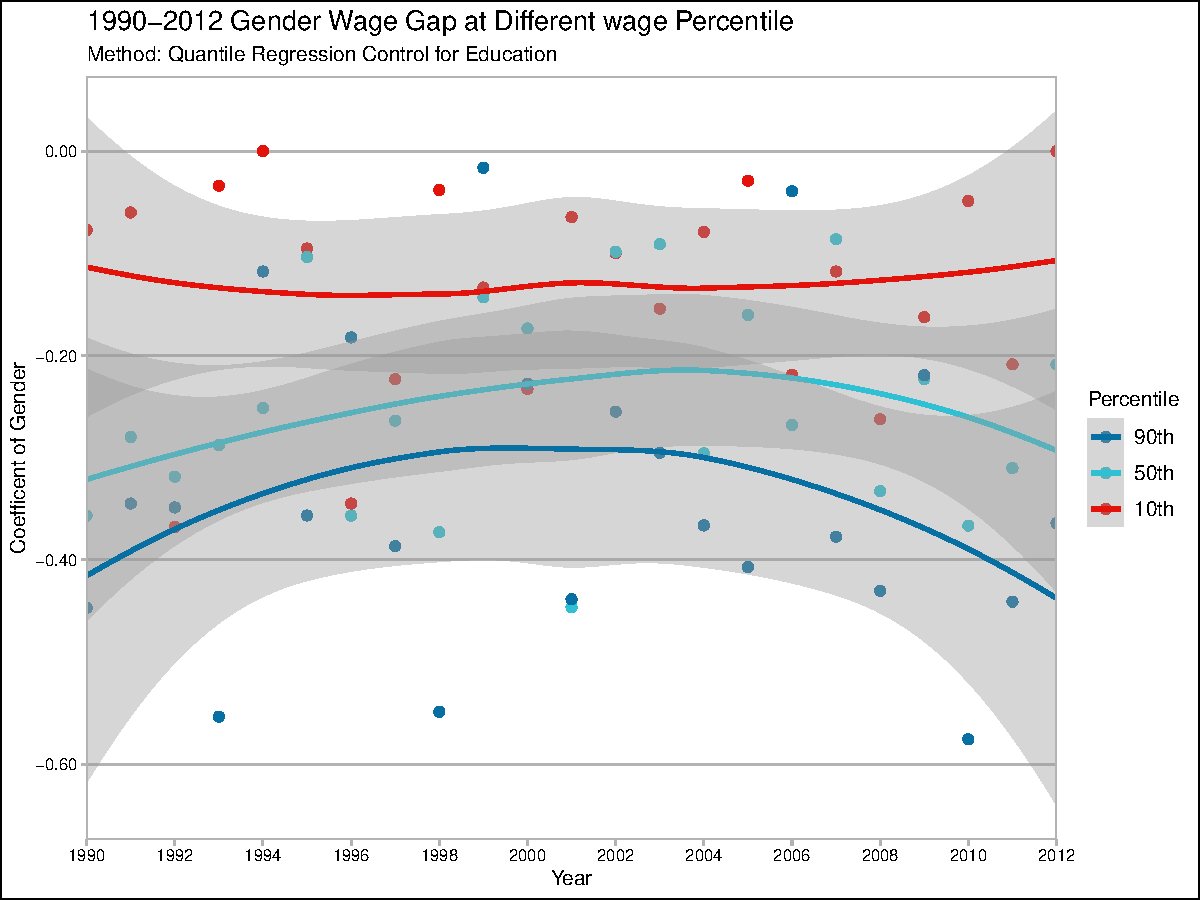
\includegraphics[width=110mm,scale=0.9]{q7p3.pdf}
    \caption{1990 - 2012 Return to education(Quantile regression)}
    \label{fig:my_label}
\end{figure}

To testify further the impact of education on different gender at different percentile,  we can use quantile regression again to see how the return to education vary over these years among different group.
\begin{equation}
    LogWage_{iqtg}=\beta_0+\beta_{2qtg}SomeUni_{iqtg}+u_{iqtg}
\end{equation}
From figure 7 and figure 8, which are respectively for male and female, we can see that the overall return to education has been decreased over time for 10th and 50th of all people, whilst the return to university attendance are still increasing, especially for women who earn a 90th quantile wage in.
\begin{figure}[H]
    \centering
    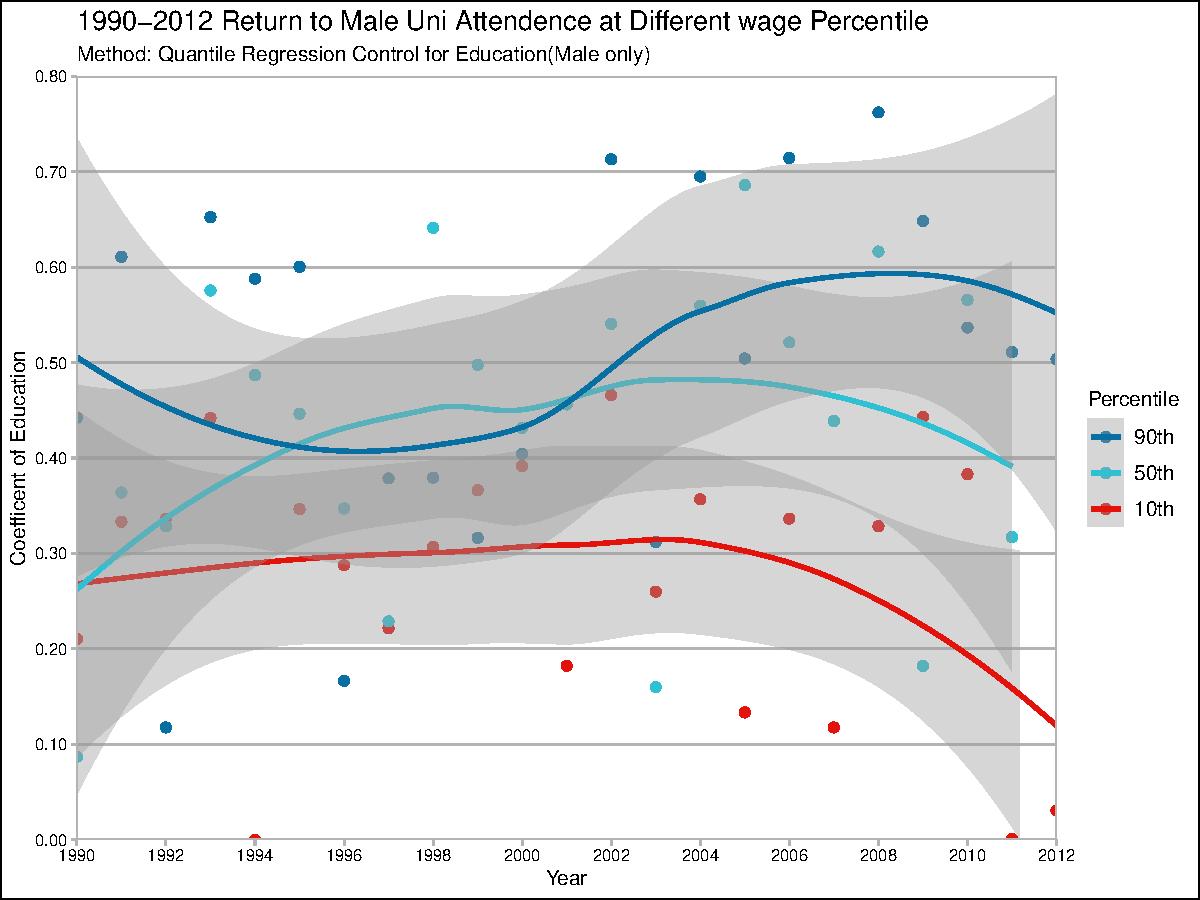
\includegraphics[width=120mm,scale=0.9]{q7p4.pdf}
    \caption{1990 - 2012 Male Return to Education(Quantile Regression)}
    \label{fig:my_label}
\end{figure}

\begin{figure}[H]
    \centering
    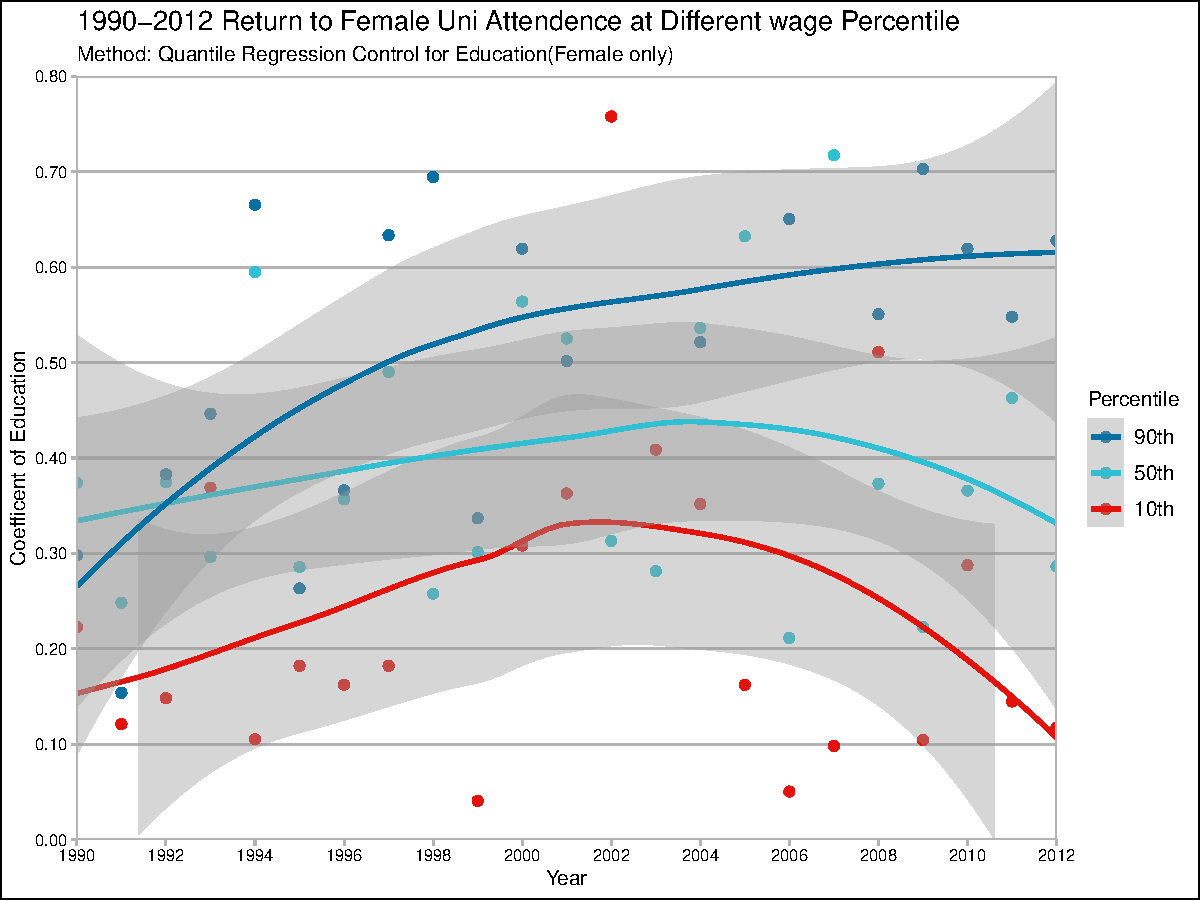
\includegraphics[width=120mm,scale=0.9]{q7p5.pdf}
    \caption{1990 -2010 Female Return to Education(Quantile Regression)}
    \label{fig:my_label}
\end{figure}

\section{Conclusion}
With the result from \textit{4.1 Control for Education}, we can state that despite women are gaining more and more education, they still are treated unequally and received less income relatively. With result of OLS indicates women on average earn 24 percent less than the man, whilst the quantile regression shows that for women in 10th percentile, they earn 14 percent less, for those in 50th, the number is 25 percent and for those in 90th, it is 35 percent.\\~\\
With the result from \textit{4.2 Gender Wage Over Time}, it can be inferred from the OLS result that gender wage gap doesn't show an expected decreasing trend, as more women are obtaining the education. Meanwhile, the return to education has been drastically decreased. However, the result of quantile regression shows that the inequality maintain the same for women who has low income job, but a larger wage gap for women who earn more(50th, 90th).\\~\\
However, a possible policy solution is to continue providing women with more education, suggested by the regression result which shows that women enjoy larger return to education(especially people at 90th), 



\end{document}
